%!TEX root = ../zeeman.tex
\subsection{Теоретический расчет расщепления линий}
Для 585.25 нм:

$$J \rightarrow J+1$$
$$J_1=0 \Rightarrow M_1=0$$
$$J_2=1 \Rightarrow M_2 =1, 0, -1$$
\begin{figure}[H]
	\centering
	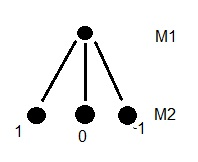
\includegraphics[width=0.3\linewidth]{fig/fig12}
	\caption{}
	\label{fig:fig12}
\end{figure}

Интенсивность:

\begin{tabular}{ | l | l | l | l |}
\hline
$\text{Поперечный эффект}$ & $ $ & $\text{Продольный эффект}$ & $ $ \\ \hline
$0 \rightarrow -1$ & $\frac12$ & $0 \rightarrow -1$ & $1$\\
$0 \rightarrow 0$ & $1$ & $0 \rightarrow 1$ & $1$\\
$0 \rightarrow 1$ & $\frac12$ & $ $ & $ $\\
\hline
\end{tabular}

\begin{tabular}{ | l | l | l | l |}
\hline
$ $ & $0 \rightarrow -1$ & $0 \rightarrow 0$ & $0 \rightarrow 1$ \\
$\Delta \omega$ & $-1$ & $0$ & $1$ \\
$\text{Поляризация}$ & $\sigma$ & $\pi$ & $\sigma$\\
$\text{Интенсивность}$ & $\frac12$ & $1$ & $\frac12$\\
\hline
\end{tabular}

Для 594.48 нм:

$$J \rightarrow J$$
$$J_1=2 \Rightarrow M_1=2,1,0,-1,-2$$
$$J_2=2 \Rightarrow M_1=2,1,0,-1,-2$$
\begin{figure}[H]
	\centering
	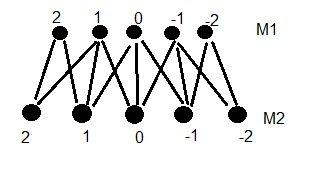
\includegraphics[width=0.3\linewidth]{fig/fig13}
	\caption{}
	\label{fig:fig13}
\end{figure}

Интенсивность:

\begin{tabular}{ | l | l | l | l |}
\hline
$\text{Поперечный эффект}$ & $ $ & $\text{Продольный эффект}$ & $ $ \\ \hline
$2 \rightarrow 2$ & $4$ & $2 \rightarrow 1$ & $2$\\
$2 \rightarrow 1$ & $1$ & $1 \rightarrow 2$ & $2$\\
$1 \rightarrow 2$ & $1$ & $1 \rightarrow 0$ & $3$\\
$1 \rightarrow 1$ & $1$ & $0 \rightarrow 1$ & $3$\\
$1 \rightarrow 0$ & $\frac32$ & $0 \rightarrow -1$ & $3$\\
$0 \rightarrow 1$ & $\frac32$ & $-1 \rightarrow 0$ & $3$\\
$0 \rightarrow 0$ & $0$ & $-1 \rightarrow -2$ & $2$\\
$0 \rightarrow -1$ & $\frac32$ & $-2 \rightarrow -1$ & $2$\\
$-1 \rightarrow 0$ & $\frac32$ & $ $ & $ $\\
$-1 \rightarrow -1$ & $1$ & $ $ & $ $\\
$-1 \rightarrow 2$ & $1$ & $ $ & $ $\\
$-2 \rightarrow -1$ & $1$ & $ $ & $ $\\
$-2 \rightarrow -2$ & $4$ & $ $ & $ $\\
\hline
\end{tabular}

\begin{tabular}{ | l | l | l | l | l | l | l | l | l |}
\hline
$ $ & $2 \rightarrow 2$ & $2 \rightarrow 1$ & $1 \rightarrow 2$ & $1 \rightarrow 1$ & $1 \rightarrow 0$ & $0 \rightarrow 1$ & $0 \rightarrow 0$ & $0 \rightarrow -1$ \\ 
$\Delta \omega$ & $0$ & $\frac32$ & $-\frac32$ & $0$ & $\frac32$ & $-\frac32$ & $0$ & $\frac32$\\ 
$\text{Поляризация}$ & $\pi$ & $\sigma$ & $\sigma$ & $\pi$ & $\sigma$ & $\sigma$ & $\pi$ & $\sigma$\\
$\text{Интенсивность}$ & $4$ & $1$ & $1$ & $1$ & $\frac32$ & $\frac32$ & $0$ & $\frac32$ \\
\hline
\end{tabular}

\begin{tabular}{| l | l | l | l | l | l | l | l |}
\hline
$-1 \rightarrow 0$ & $-1 \rightarrow -1$ & $-1 \rightarrow -2$ & $-2 \rightarrow -1$ & $-2 \rightarrow -2$\\
$-\frac32$ & $0$ & $\frac32$ & $-\frac32$ & $0$\\
$\sigma$ & $\pi$ & $\sigma$ & $\sigma$ & $\pi$\\
$\frac32$ & $1$ & $1$ & $1$ & $4$\\
\hline
\end{tabular}

Для 607.4 нм:

$$J \rightarrow J+1$$
$$J_1=0 \Rightarrow M_1=0$$
$$J_2=1 \Rightarrow M_1=1,0,-1$$
\begin{figure}[H]
	\centering
	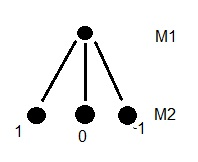
\includegraphics[width=0.3\linewidth]{fig/fig12}
	\caption{}
	\label{fig:fig14}
\end{figure}
Интенсивность:

\begin{tabular}{ | l | l | l | l |}
\hline
$\text{Поперечный эффект}$ & $ $ & $\text{Продольный эффект}$ & $ $ \\ \hline
$0 \rightarrow -1$ & $\frac12$ & $0 \rightarrow -1$ & $1$\\
$0 \rightarrow 0$ & $1$ & $0 \rightarrow 1$ & $1$\\
$0 \rightarrow 1$ & $\frac12$ & $ $ & $ $\\
\hline
\end{tabular}

\begin{tabular}{ | l | l | l | l |}
\hline
$ $ & $0 \rightarrow 1$ & $0 \rightarrow 0$ & $0 \rightarrow -1$ \\
$\Delta \omega$ & $-\frac32$ & $0$ & $\frac32$ \\
$\text{Поляризация}$ & $\sigma$ & $\pi$ & $\sigma$\\
$\text{Интенсивность}$ & $\frac12$ & $1$ & $\frac12$\\
\hline
\end{tabular}

Для 638.3 нм:

$$J \rightarrow J$$
$$J_1=1 \Rightarrow M_1=1,0,-1$$
$$J_2=1 \Rightarrow M_1=1,0,-1$$
\begin{figure}[H]
	\centering
	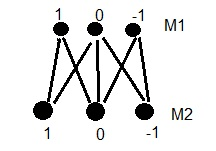
\includegraphics[width=0.3\linewidth]{fig/fig14}
	\caption{}
	\label{fig:fig15}
\end{figure}

Интенсивность:

\begin{tabular}{ | l | l | l | l |}
\hline
$\text{Поперечный эффект}$ & $ $ & $\text{Продольный эффект}$ & $ $ \\
$1 \rightarrow 1$ & $1$ & $1 \rightarrow 0$ & $1$\\
$1 \rightarrow 0$ & $\frac12$ & $0 \rightarrow 1$ & $1$\\
$0 \rightarrow 1$ & $\frac12$ & $0 \rightarrow -1$ & $1$\\
$0 \rightarrow 0$ & $0$ & $-1 \rightarrow 0$ & $1$\\
$0 \rightarrow -1$ & $\frac12$ & $ $ & $1$\\ 
$-1 \rightarrow 0$ & $\frac12$ & $ $ & $1$\\
$-1 \rightarrow 1$ & $1$ & $ $ & $ $\\
\hline
\end{tabular}

\begin{tabular}{ | l | l | l | l | l | l | l | l |}
\hline
$ $ & $1 \rightarrow 1$ & $1 \rightarrow 0$ & $0 \rightarrow 1$ & $0 \rightarrow 0$ & $0 \rightarrow -1$ & $-1 \rightarrow 0$ & $-1 \rightarrow -1$\\ 
$\Delta \omega$ & $-1$ & $\frac12$ & $-\frac32$ & $0$ & $\frac32$ & $-\frac12$ & $1$\\ 
$\text{Поляризация}$ & $\pi$ & $\sigma$ & $\sigma$ & $\pi$ & $\sigma$ & $\sigma$ & $\pi$\\
$\text{Интенсивность}$ & $1$ & $\frac12$ & $\frac12$ & $0$ & $\frac12$ & $\frac12$ & $1$ \\
\hline
\end{tabular}

\subsection{Наблюдение нормального эффекта Зеемана}
На примере линии 585.25 нм.
Характер поляризации компонент при поперечном эффекте:
\begin{figure}[H]
	\centering
	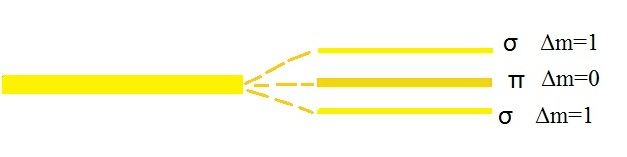
\includegraphics[width=0.5\linewidth]{fig/fig15}
	\caption{}
	\label{fig:fig16}
\end{figure}

Расщепление в поперечном эффекте при значении магнитного поля $H=6100 \text{ эрстед} (1.8 A)$.
\begin{figure}[H]
	\centering
	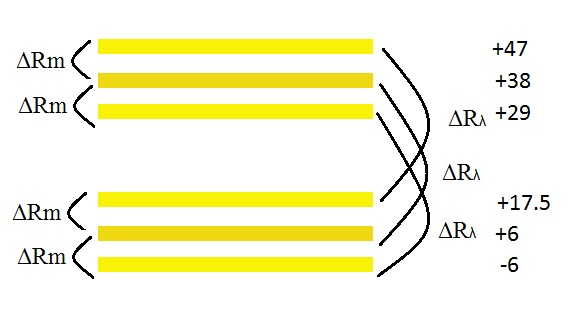
\includegraphics[width=0.5\linewidth]{fig/fig16}
	\caption{}
	\label{fig:fig17}
\end{figure}

Удельный заряд электрона $\frac{e}{m} = \frac{2c^2d\lambda}{\lambda^2 H}$

$\frac{e}{m}_{\text{прак}} = 0.12\cdot10^{18}$, $\frac{e}{m}_{\text{теор}} = 0.52\cdot 10^{18}$.

Разрешающая способность ИФП  при $H=4400 \text{ эрстед} (1 A)$ ($\rho=0.89, m_i=m_0=\frac{2h}{\lambda}$)

$$R_{\text{теор}}=\frac{m_i \pi \sqrt{\rho}}{1-\rho}= 368 900$$
$$R_{\text{прак}}=\frac{\omega}{\Delta \omega}= 82 200$$ 

\subsection{Изучение аномального эффекта Зеемана}
На примере линии 607.4 нм.
Характер поляризации компонент при поперечном эффекте:
\begin{figure}[H]
	\centering
	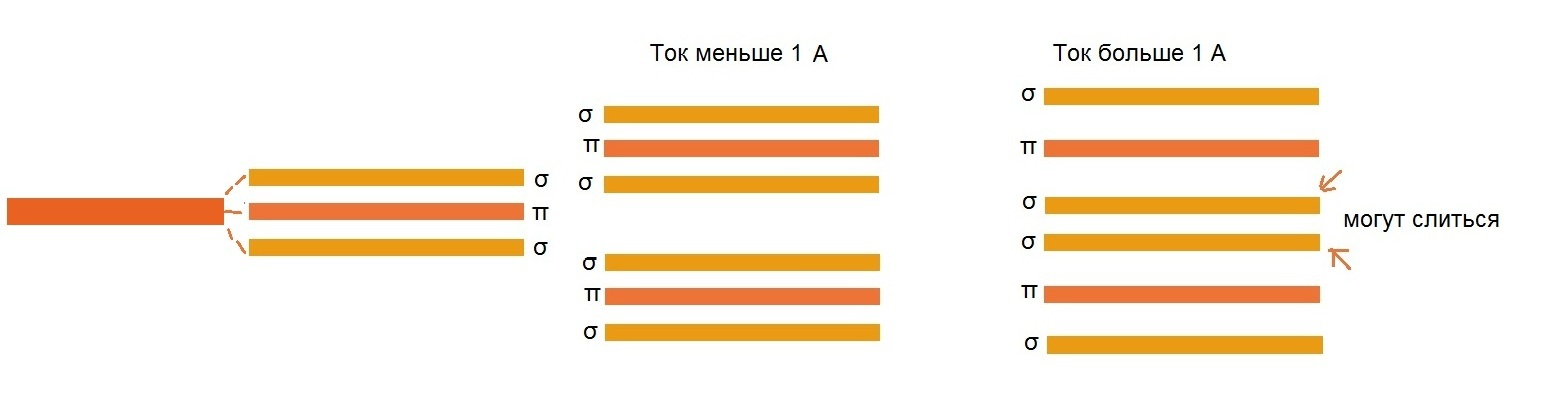
\includegraphics[width=\linewidth]{fig/fig17}
	\caption{}
	\label{fig:fig18}
\end{figure}

Расщепление в поперечном эффекте при значении магнитного поля $H=4400 \text{ эрстед} (1 A)$.
\begin{figure}[H]
	\centering
	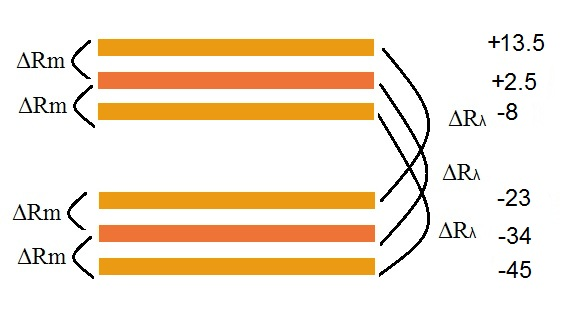
\includegraphics[width=0.5\linewidth]{fig/fig18}
	\caption{}
	\label{fig:fig19}
\end{figure}

разность g-факторов: $1.8 \pm 0.1$.

\subsection{Изучение аномального зеемановского расщепления при наличии более чем трех разрешаемых прибором компонент}
На примере линии 638.3 нм.
\begin{figure}[H]
	\centering
	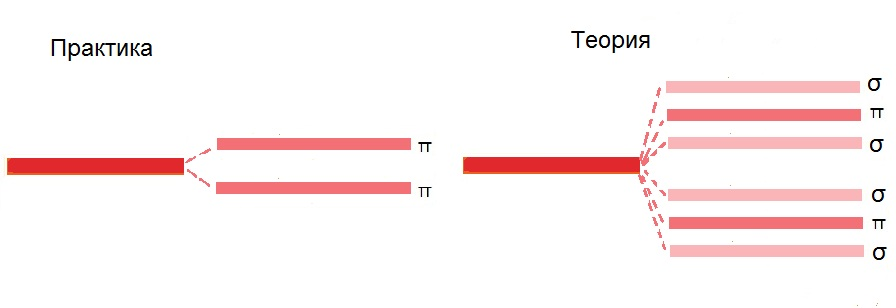
\includegraphics[width=0.8\linewidth]{fig/fig19}
	\caption{}
	\label{fig:fig20}
\end{figure}

Расщепление компонент
\begin{figure}[H]
	\centering
	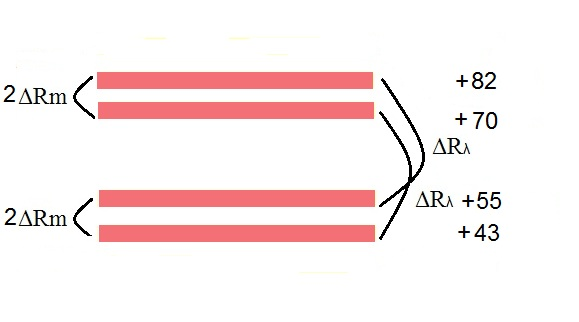
\includegraphics[width=0.5\linewidth]{fig/fig20}
	\caption{}
	\label{fig:fig21}
\end{figure}

разность g-факторов: $1.35 \pm 0.1$.

\subsection{Изучение аномального эффекта Зеемана в условиях частичного разрешения компонент}
На примере линии 594.48 нм.
\begin{figure}[H]
	\centering
	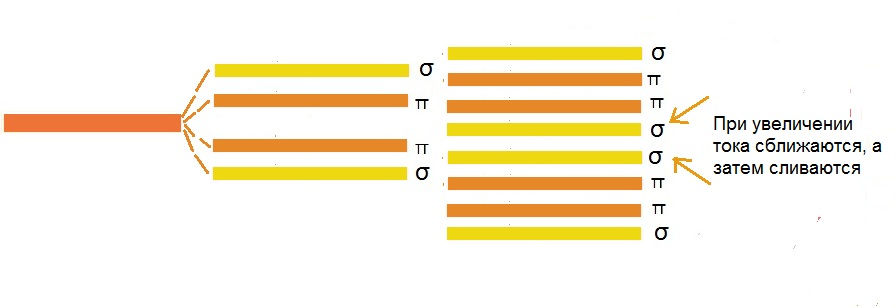
\includegraphics[width=0.8\linewidth]{fig/fig21}
	\caption{}
	\label{fig:fig22}
\end{figure}

Ток, при котором полосы еще различимы $I=2.35 A$. 

\section{Вывод}
В ходе эксперимента изучена теория простого и сложного эффектов Зеемана, исследован характер поляризации компонент в поперечном магнитном поле. Получено значение удельного заряда электрона $\frac{e}{m}_{\text{прак}} = 0.12\cdot10^{18}$, совпадающего по порядку с теоретическим. Оценена разрешающая способность ИФП $R_{\text{прак}}=\frac{\omega}{\Delta \omega}= 82 200$. Определены разности g-факторов для случая аномального эффекта. 
